\documentclass{article}
\PassOptionsToPackage{round,authoryear}{natbib}
\usepackage[dblblindworkshop]{neurips_2026}
\workshoptitle{Neural Network Artifacts as a New Data Modality}

\usepackage[utf8]{inputenc}
\usepackage[T1]{fontenc}
\usepackage{hyperref}
\usepackage{url}
\usepackage{booktabs}
\usepackage{amsmath,amssymb}
\usepackage{amsfonts}
\usepackage{amsthm}
\usepackage{microtype}
\usepackage{graphicx}

\newtheorem{lemma}{Lemma}

\title{Behavioural Traces as Neural Artifacts: An Exact Null for Model Populations, and Lineage Recovery Without Weights}

\author{
  Anonymous Author(s) \\
  Affiliation \\
  Address \\
  \texttt{email}
}

\begin{document}

\maketitle

\begin{abstract}
Learning from populations of neural artifacts has so far meant learning from weights, gradients and
internal traces. For most of the open model ecosystem none of those are practically available at
population scale, but one artifact always is: the record of which benchmark items a model gets
wrong. We argue this behavioural trace deserves treatment as an artifact modality in its own right,
and we supply the three things such a modality needs. First, a released model zoo: per-item outcome
matrices for $1{,}228$--$4{,}562$ open models across five benchmarks, harvested from archived
evaluation files at zero inference cost, with the two identifier pitfalls that make a naive harvest
return an empty join documented and guarded. Second, an exact null. We show the obvious
population-level statistic, mean pairwise co-failure, is a deterministic function of item difficulty
alone and therefore carries no information about model relatedness whatsoever, and that the row and
column margins of the outcome matrix are the jointly sufficient statistics of the Rasch family, so
the uniform distribution over margin-matched matrices is a fit-free conditional null that removes
item difficulty exactly. Third, evidence the modality carries provenance: after conditioning, a
$5$-nearest-neighbour classifier on the leading residual eigenvectors recovers a model's base family
with leave-one-out accuracy $0.807$ over $916$ labelled models from five families, against a
label-permutation null of $0.287\pm0.017$ and a majority-class rate of $0.382$, while the same
pipeline run on a draw from the exact null returns $0.318$, at chance. We report the controls that
weaken the strongest reading as prominently as the result, including that unconditioned
eigenvectors already reach $0.760$, so conditioning is not what creates the signal.
\end{abstract}

\section{Introduction}

Model repositories now hold hundreds of thousands of trained networks, and a growing body of work
treats that population as data: learning on weights, merging models, predicting properties from
parameters, mapping model atlases. The premise is that a trained model leaves artifacts, and that
populations of artifacts can be compared, searched and explained.

That premise has an access problem which the weight-centric framing does not solve. Weights are
downloadable in principle and prohibitive in practice at population scale; gradients, optimization
trajectories and internal representations require running the model, which for thousands of models
is a serious compute bill; and for any model behind an API, none of the four exists. What does
exist, for every model anyone has ever evaluated, is the record of which items it got wrong. Public
leaderboards have been accumulating exactly this for years, item by item, model by model, and it is
readable without loading a single weight.

We take that record seriously as an artifact modality. A model's per-item outcome vector is a
computational trace: it is a projection of the weights through a fixed probe set, lossy but
faithful, and cheap enough that a population of thousands is a file read rather than a compute job.
The question this paper asks is whether that trace supports the things this community wants from
artifacts, and specifically whether it carries \emph{neural lineage}.

\paragraph{Contributions.}
\begin{enumerate}
\item \textbf{A model zoo in the behavioural-trace modality} (Section~\ref{sec:data}):
per-item binary outcome matrices for five benchmarks over $1{,}228$--$4{,}562$ models each, with
the harvest procedure, the two identifier pitfalls that silently break it, and the row-order audit
that licenses the join.
\item \textbf{An exact, fit-free null for population-level analysis of these artifacts}
(Section~\ref{sec:null}). We prove the first statistic anyone computes is degenerate, identify the
canonical null from Rasch sufficiency, and validate the sampler against exhaustive enumeration
rather than asserting it.
\item \textbf{A calibrated measurement of residual structure} across the five benchmarks
(Section~\ref{sec:structure}), together with a negative result about the statistic most tempting to
report.
\item \textbf{Lineage recovery from behavioural traces alone} (Section~\ref{sec:lineage}):
family classification at $0.807$ against a $0.287$ permutation null, with five pre-registered
controls, including two that cut against the strongest reading.
\item \textbf{A monitor for a growing population} (Section~\ref{sec:monitor}), since a model zoo
harvested from a live archive is not a fixed dataset.
\end{enumerate}

\section{Related work}

Learning from populations of neural artifacts has largely meant learning from weights.
\citet{unterthiner2021} showed a trained network's accuracy is predictable from simple weight
statistics without evaluating it on data, and released $120$k CNNs to support the task;
\citet{schurholt2022} published systematically generated model zoos as a dataset in their own
right. Our zoo is complementary in construction and in cost: it is not generated but harvested, the
models are the ecosystem's actual submissions rather than a controlled sweep, and the artifact is a
behavioural trace, which is available for models whose weights are impractical to collect or absent
entirely. The trade is real in both directions --- weights support parameter-space operations such
as merging and editing that a trace cannot, while a trace is obtainable at population scale for
essentially free and is architecture-agnostic by construction.

Closest to our lineage result is the model atlas of \citet{horwitz2025}, who chart Hugging Face's
documented lineage graph, demonstrate applications including attribute prediction, and, because
``most models are poorly documented'', propose recovering undocumented regions from structural
priors on real-world training practice. We attack the same documentation gap from the opposite
side. We quantify it on our population --- a declared parent resolves for $23.3\%$ of models, with
$315$ of $1{,}362$ repositories no longer retrievable --- and then ask what can be recovered with no
documentation and no priors on training practice at all, using only behaviour. The two are
complementary: structural priors and behavioural evidence are independent sources on the same latent
graph, and a signal that recovers family at $0.807$ from traces is a candidate edge weight for
exactly the undocumented regions an atlas cannot yet chart.

Methodologically, the exact conditional null we use is standard in ecology
\citep{schluter1984,gotelli2000,strona2014} and psychometrics
\citep{rasch1960,andersen1973,fleiss1971}, and the degeneracy of the mean statistic is known
independently in both plus the classifier-ensemble literature \citep{kuncheva2003,cronbach1951}.
None of it appears in the artifact-population literature, and importing it is a large part of what
this paper is for.

\section{The artifact and the zoo}
\label{sec:data}

Let $F\in\{0,1\}^{N\times M}$ with $F_{im}=1$ iff model $i$ fails item $m$; row sums $r_i$, column
sums $c_m$. One row is one model's behavioural trace on one probe set.

We harvest $F$ from the archived Open LLM Leaderboard. Only the metric column of each result file
is read --- $1.4$\,KB out of a $63$\,MB file for HellaSwag --- which is what makes an
ecosystem-scale harvest possible at zero inference cost.

\paragraph{Two pitfalls, documented because they are silent.} Item identifiers are not stable
across the archive: the harness stored a dataset identifier in mid-2023 and the raw question text
thereafter, so a naive identifier join returns an \emph{empty} intersection rather than a wrong
one. The accuracy field also moved into a nested \texttt{metrics} struct in the 2024 schema. We
resolve item identity by row index, licensed by explicit verification rather than assumption:
across all five benchmarks, row order was identical for every one of $334$ models sampled evenly
over July 2023 to May 2024, with zero mismatches (ARC $149/149$, TruthfulQA $60/60$, GSM8K $60/60$,
Winogrande $40/40$, HellaSwag $25/25$), and a row-count guard runs on every read. An undetected
misalignment would make a model's row look independent of every other and so bias correlations
\emph{toward} the null, understating rather than manufacturing any result below.

\begin{table}[t]\centering\small
\begin{tabular}{lrrrrr}
\toprule
& \multicolumn{2}{c}{frozen analysis set} & \multicolumn{2}{c}{current release} & \\
\cmidrule(lr){2-3}\cmidrule(lr){4-5}
Benchmark & models & items & models & items & mean accuracy \\
\midrule
ARC-Challenge & 1362 & 1165 & 4562 & 1170 & 0.527 \\
Winogrande & 1361 & 1267 & 4544 & 1267 & 0.734 \\
TruthfulQA (mc1) & 1334 & 786 & 3531 & 811 & 0.368 \\
GSM8K & 1228 & 1319 & 3405 & 1319 & 0.348 \\
HellaSwag & 1362 & 9404 & 2972 & 9802 & 0.581 \\
\bottomrule
\end{tabular}
\caption{The zoo. Counts are after removing rows and columns that are all-correct or all-wrong;
mean accuracy is over the full pre-filter matrix. The archive is live and a scheduled process keeps
harvesting it, so the two column groups differ: every analysis below names the snapshot it used and
the release pins each by content hash.}
\label{tab:zoo}
\end{table}

\paragraph{The zoo is not static, and this matters.} A population harvested from a live archive
grows underneath the analysis. Between the frozen set and the current release, ARC grew from
$1{,}362$ to $4{,}562$ models; one harvest landed during the preparation of this paper. Every
number below is therefore labelled with its snapshot, and each snapshot is identified in the
released artifacts by the SHA-256 of the matrix file, which is what makes a run reproducible when
the underlying archive will not hold still. We think any benchmark or dataset in this modality
needs the same discipline, and note it as a small proposal for the community's dataset practice.

\section{Why population-level analysis of these artifacts needs a null}
\label{sec:null}

The natural first question about a population of traces is how often two models fail together. That
statistic is uninformative, and provably so.

\begin{lemma}[Mean co-failure depends only on item margins]
\label{lem:mean}
The mean pairwise co-failure rate is
$O=\frac{1}{N(N-1)}\sum_{i\neq j}\frac1M\sum_m F_{im}F_{jm}=\frac{1}{MN(N-1)}\sum_m (c_m^2-c_m)$.
\end{lemma}
\begin{proof}
$\sum_{i\neq j}F_{im}F_{jm}=(\sum_i F_{im})^2-\sum_i F_{im}^2=c_m^2-c_m$ since $F_{im}\in\{0,1\}$.
\end{proof}

\noindent $O$ is a function of the item margins alone, so any randomization that preserves them
leaves it invariant with exactly zero variance: the ``excess'' co-failure over such a null is
identically zero by construction, not empirically small. Mean pairwise disagreement inherits the
degeneracy, being $2\bar p - 2O$. The same identity is Schluter's V-ratio in ecology
\citep{schluter1984,gotelli2000}, Cronbach's $\alpha$ in psychometrics \citep{cronbach1951}, and
Fleiss's observed agreement in the multi-category case \citep{fleiss1971}; it is also the
double-fault diversity measure of the classifier-ensemble literature \citep{kuncheva2003}. We
restate rather than claim it, because a population-level artifact study that reports mean
co-failure is reporting item difficulty.

\paragraph{The canonical null.} The Rasch model $\Pr(F_{im}=1)=\sigma(\alpha_i+\beta_m)$ has
$\{r_i\}$ and $\{c_m\}$ as jointly sufficient statistics, so the conditional law of $F$ given its
margins is uniform on the set of margin-matched binary matrices, for every parameter value
\citep{rasch1960,andersen1973}. That set is the ecologists' fixed-fixed null. Conditioning on it
removes model ability and item difficulty exactly, without an optimizer, a penalty, or an
identification convention --- which matters here because the alternative, fitting an item-response
model to each population, introduces analyst choices that a population study should not have to
defend.

\paragraph{Sampling it, verified rather than asserted.} We sample with curveball
\citep{strona2014}, whose convergence to uniform on the fibre requires that failed trades count as
steps \citep{carstens2015}; ours does. We test it directly: enumerating every binary matrix with
given margins on four small fibres (sizes $48$, $90$, $204$, $1{,}170$) and drawing $60{,}000$
thinned samples, a $\chi^2$ test against uniformity is not rejected on any
($p=0.23,\,0.05,\,0.73,\,0.15$). On the real matrices, four dispersed chains give Gelman--Rubin
$\hat R\in[0.98,1.03]$ at the burn-in used.

\paragraph{Statistics.} Let $P$ be the Rasch mean field matching the observed margins (fitted to
margin error below $10^{-11}$), $D=(FF^{\!\top}-PP^{\!\top})/M$, and $R$ the unit-diagonal scaling
of $D$. We report the rms off-diagonal $|R_{ij}|$, the participation ratio
$\mathrm{PR}=(\sum_k\lambda_k^{+})^2/\sum_k(\lambda_k^{+})^2$ of $R$'s positive spectrum, and the
count of eigenvalues of $R$ above the null's largest --- parallel analysis against the exact null
rather than against iid noise. Each is compared to the same quantity on margin-matched replicates.
$P$ is validated against the randomization itself: over $319{,}600$ ARC model pairs, the curveball
expectation of $\frac1M\sum_m F_{im}F_{jm}$ and the Rasch prediction correlate at $0.99999$.

\section{What the null reveals}
\label{sec:structure}

\begin{table}[t]\centering\small
\begin{tabular}{lrrrrrrr}
\toprule
& & \multicolumn{3}{c}{rms $|R_{ij}|$} & \multicolumn{2}{c}{participation ratio} & \\
\cmidrule(lr){3-5}\cmidrule(lr){6-7}
Benchmark & $N$ & obs. & null & ratio & obs. & null & dims $>$ edge \\
\midrule
ARC-Challenge & 1362 & 0.2483 & 0.0449 & $5.5\times$ & 23.6 & $449.3\pm3.4$ & 6 \\
Winogrande & 1361 & 0.2691 & 0.0409 & $6.6\times$ & 20.1 & $493.8\pm3.0$ & 5 \\
TruthfulQA & 1334 & 0.2942 & 0.0583 & $5.1\times$ & 17.4 & $309.7\pm2.4$ & 5 \\
GSM8K & 1228 & 0.0987 & 0.0346 & $2.9\times$ & 118.6 & $553.1\pm2.2$ & 4 \\
HellaSwag & 1362 & 0.2457 & 0.0206 & $11.9\times$ & 27.3 & $958.0\pm3.2$ & 12 \\
\bottomrule
\end{tabular}
\caption{Residual structure on the frozen analysis set after exact-margin conditioning. Null rms is
the mean over $40$ curveball replicates; null PR is mean $\pm$ SD over $60$ independent-chain
replicates, both margins exactly preserved at every draw.}
\label{tab:structure}
\end{table}

Table~\ref{tab:structure} reports what survives conditioning. Residual correlation runs
$2.9$--$11.9\times$ its null and the participation ratio sits at $2.8$--$21.4\%$ of its null on
every benchmark. Before conditioning, the same participation ratio reads $1.5$--$3.6$ on all five,
a number driven almost entirely by the single shared item-difficulty eigenvalue that conditioning
removes: uncalibrated, the modality looks like it contains almost no independent models, which is
an artifact of the statistic rather than a property of the population.

\paragraph{A negative result about the tempting statistic.} It is tempting to read
Table~\ref{tab:structure} as ``$1{,}362$ models behave like $24$''. That reading is wrong for an
algebraic reason worth stating in this venue, because the participation ratio is a natural summary
for any artifact population. For the unclipped spectrum,
$\mathrm{PR}=N/(1+(N-1)\overline{R_{ij}^2})$ exactly --- $16.04$ on ARC computed either way --- so
PR is a monotone transform of mean squared residual correlation and the eigendecomposition
contributes nothing. An equicorrelated matrix and a partition into $24$ tight clusters give the same
value. The statistic cannot license a count of independent models, and we report it only as a
calibrated summary. The diagnostics that \emph{can} separate those cases say the ARC structure is
neither: the leading eigenvalue carries $54\%$ of squared residual mass (one shared factor would
give $\approx99\%$, twenty clone blocks $\approx10\%$), deflating it raises PR only to $46.8$
rather than toward $N$, and six eigenvalues clear the null's spectral edge.

\paragraph{What else could produce this.} Each row below is a simulated population with no clusters,
no clones and no shared lineage --- errors conditionally independent given the item.

\begin{table}[t]\centering\small
\begin{tabular}{lrrrr}
\toprule
Generating process & PR / PR$_{\text{null}}$ & rms $|R_{ij}|$ & $\lambda_1^2/\sum\lambda^2$ & dims $>$ edge \\
\midrule
1PL, correctly specified & $1.001$ & $0.065$ & $0.105$ & 1 \\
2PL, $\mathrm{sd}(\log a)=0.35$ & $0.966$ & $0.068$ & $0.119$ & 1 \\
2PL, $\mathrm{sd}(\log a)=0.60$ & $0.862$ & $0.076$ & $0.167$ & 1 \\
two ability dimensions & $0.230$ & $0.162$ & $0.457$ & 3 \\
20 exact clone clusters & $0.112$ & $0.234$ & $0.102$ & 19 \\
\midrule
\textbf{real ARC} & $\mathbf{0.052}$ & $\mathbf{0.248}$ & $\mathbf{0.540}$ & \textbf{6} \\
\bottomrule
\end{tabular}
\caption{Discrimination heterogeneity alone cannot reproduce the observed effect. A low-dimensional
multi-ability structure reproduces much of it, and the observed spectral signature resembles that
case rather than duplicated models.}
\label{tab:misspec}
\end{table}

Two readings follow, and the second is a limitation. Discrimination heterogeneity is not a
sufficient explanation: even at $\mathrm{sd}(\log a)=0.60$ it yields rms $0.076$ against the
observed $0.248$. But a small number of extra ability dimensions is a substantial one, and the
observed $\lambda_1^2/\sum\lambda^2=0.540$ sits near the two-dimensional case ($0.457$) and far
from the clone case ($0.102$). We therefore cannot separate ``genuine behavioural concentration''
from ``the conditioning family is too small'', and on the spectral evidence the latter is the
better description.

\paragraph{Robustness.} Recomputing every statistic on populations deduplicated at pairwise
agreement $0.95$, discarding $21$--$64\%$ of models with the Rasch fit and null redrawn each time,
moves $14$ of $15$ statistic--benchmark pairs by at most $1.5\times$; the exception is HellaSwag's
PR ratio at $2.44\times$. On planted data the test reaches power $1.00$ against shared failure modes
at a planted rms of $0.048$, far below the $0.099$--$0.294$ observed, and rejects at $0.017$ under
the null. Against the alternative in which every model shares one item-difficulty profile and
differs only in ability, power is exactly $\alpha$ --- that alternative \emph{is} the null, and we
report the blind spot as a property of the design rather than a caveat. Two candid points about the
null itself: its rms sits only $1.25$--$2.01\times$ above the analytic $1/\sqrt{M}$ floor, and
conditioning on item margins alone reproduces the both-margin null to within $8.3\%$ on every
benchmark, so the item margins do essentially all of the conditioning work for this statistic.

\section{A second trace modality: which wrong answer}
\label{sec:multicat}

Binary correctness is the coarsest reading of a behavioural trace. The archive also records
per-choice log-likelihoods for part of the population, from which the model's \emph{chosen} answer
is recoverable, giving a multi-category trace: not whether a model failed, but how. Analysts use it
to ask whether models make the same mistakes. That statistic has its own degeneracy, and the same
conditioning idea repairs it.

\begin{lemma}[Agreement given both wrong depends only on per-item response composition]
\label{lem:fleiss}
Let $n_{mk}$ be the number of models choosing option $k$ on item $m$ and $n_m=\sum_k n_{mk}$. The
mean pairwise same-answer rate is
$A=\left.\sum_m\sum_k n_{mk}(n_{mk}-1)\middle/\sum_m n_m(n_m-1)\right.$,
a function of the per-item composition $\{n_{mk}\}$ alone. Any relabelling of which model gave
which recorded answer, item by item, leaves $A$ exactly invariant with zero variance.
\end{lemma}

\noindent This is Fleiss's observed agreement \citep{fleiss1971} and the founding premise of
answer-copying detection in psychometrics. It matters here because it is easy to demonstrate
constructively: in a simulation where models err \emph{conditionally independently} given the item,
drawing from a shared per-item distractor-attractiveness distribution, agreement-given-both-wrong is
$0.5567$ against a uniform baseline of $0.3333$ --- an apparent excess of $+0.2233$ that looks like
shared behaviour and is not --- while the excess over the composition-preserving null implied by
Lemma~\ref{lem:fleiss} is $-1.1\times10^{-16}$. Independent models, large apparent error
correlation, purely from the distractor structure of the probe set.

\paragraph{The critique does not always bite, and we report where it does not.} A degeneracy result
invites the conclusion that findings in this modality are artifacts. We tested that against a
specific published claim --- that more accurate models give more similar wrong answers --- with a
kill condition fixed in advance: if the accuracy--agreement slope survives conditioning with a
confidence interval excluding zero, the critique does not apply and the claim stands. We
reconstructed each model's chosen answer from per-choice log-likelihoods on a $600$-model ARC
subsample, recovering the gold answer from cross-model agreement (agreement among correct models
$1.0000$ on $1{,}144$ items; the recovered key reproduces each model's own reported accuracy on
$99.01\%$ of cells, which we take as validating the reconstruction rather than assuming it).

Over $38{,}238$ model pairs, the raw slope of agreement-when-both-wrong against mean pair accuracy
is $+0.585$ ($95\%$ CI $[0.577,0.594]$); conditioned on the composition-preserving null it is
$+0.514$ ($[0.506,0.522]$), an attenuation of only $12.1\%$. The kill condition fired: the claim is
not an artifact of item-level distractor composition and we report it as robust. Two things are
true at once, and both are properties of the modality worth knowing. The mean-level excess is
essentially zero --- $0.7332$ observed against $0.7324$ expected under conditional independence,
$+0.00085$, exactly as Lemma~\ref{lem:fleiss} predicts --- while the \emph{relationship} between
accuracy and agreement is not a mean-level statistic and is not absorbed by the same conditioning.
Degeneracy of a summary does not imply degeneracy of every claim built on the underlying trace, and
the way to tell is to condition and look.

\paragraph{Two opposite-looking results reconcile exactly.} A related trap: on the binary traces, a
pre-registered dispersion statistic $\operatorname{Var}_{i<j}(C_{ij})$ came out \emph{below} its
null on three of five benchmarks, while the participation ratio sits far below its null, which is
algebraically the same as residual correlations sitting far \emph{above} theirs. Both are correct.
Writing $C=E+D$ with $E=PP^{\!\top}/M$ the margin-model part,
$\operatorname{Var}(C)=\operatorname{Var}(E)+2\operatorname{Cov}(E,D)+\operatorname{Var}(D)$, and
because the null preserves margins, $\operatorname{Var}(E)$ is identical for the observation and
every replicate. On ARC, $\operatorname{Var}(D)=6.25\times10^{-4}$ against a null of
$2.13\times10^{-5}$ (a $29\times$ excess), while $\operatorname{Cov}(E,D)=-6.49\times10^{-4}$
against $-2.1\times10^{-6}$ (correlation $-0.285$ against $-0.005$). The negative covariance
outweighs the inflated variance, which is exactly why the dispersion reads low. Pairs the margin
model expects to co-fail most actually co-fail relatively less: structured deviation from
unidimensionality, which is what ``models cluster into behavioural types'' means when stated in
these terms.

\section{Neural lineage from behavioural traces}
\label{sec:lineage}

The previous section says the modality contains structure. This section asks whether that structure
is \emph{about} anything, and takes the question this workshop poses directly: can artifacts reveal
provenance?

\paragraph{Why we could not answer it with metadata.} We first tried the direct route. The
leaderboard carries an optional, self-reported \texttt{base\_model} field; on the frozen ARC set it
resolved a declared parent for $317$ of $1{,}362$ models ($23.3\%$), with $315$ repositories no
longer retrievable at all. A $40\%$ coverage threshold had been registered in advance as the point
below which a lineage decomposition would not be trusted. It fired, and the decomposition was
dropped rather than run on the surviving quarter. Declared provenance for this population does not
exist at usable coverage, which is precisely the condition under which an artifact-derived signal
would be worth having.

\paragraph{Setup.} On the pinned ARC snapshot ($N=3{,}762$, $M=1{,}169$, SHA-256
\texttt{79d2490e\ldots}), take the top-$k$ eigenvectors of $R$ with $k$ the number of eigenvalues
above the exact null's spectral edge ($k=4$, edge $79.5$). Label base family by string matching on
the model identifier against known base-model names --- a coarse lower bound on relatedness,
explicitly not lineage ground truth, reaching $34.5$--$35.7\%$ of identifiers. Use the five largest
families: $916$ models, Mistral $350$, Llama-2 $211$, Llama-3 $188$, Qwen $84$, Mixtral $83$.
Classify by leave-one-out $5$-nearest-neighbour in the standardised loading space.

\begin{figure}[t]
\centering
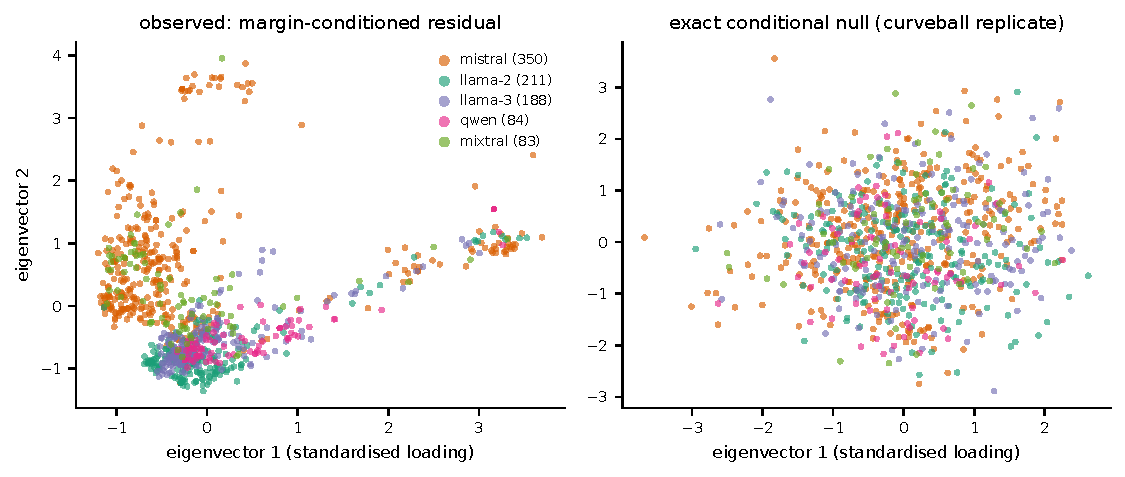
\includegraphics[width=\linewidth]{../../../figures/fig_w1_family.pdf}
\caption{Models projected on the top two residual eigenvectors, coloured by base family (left), and
the identical pipeline applied to a curveball replicate of the same matrix (right). The replicate
preserves both margins exactly and destroys any real association between behaviour and family, so
the right panel is what the left would look like if the construction were manufacturing structure.
The classifier uses four eigenvectors, not the two drawn here.}
\label{fig:family}
\end{figure}

\paragraph{Result.} Family is recovered at accuracy $\mathbf{0.807}$, against a label-permutation
null of $0.287\pm0.017$ ($1{,}000$ permutations, $p=0.001$, the resolution floor) and a
majority-class rate of $0.382$. Per-family recall is above chance for four of five: Mistral $0.926$,
Llama-2 $0.839$, Llama-3 $0.777$, Qwen $0.714$, Mixtral $0.386$. Accuracy rises monotonically with
the number of eigenvectors used --- $0.452$ at $k=1$, $0.807$ at $k=4$, $0.864$ at $k=6$, $0.905$ at
$k=20$ --- so the lineage signal is spread across many residual dimensions rather than carried by
one. Every control below was specified before the experiment ran.

\begin{table}[t]\centering\small
\begin{tabular}{llrrl}
\toprule
Arm & What it tests & Acc. & Perm. & Reading \\
\midrule
Main & residual eigenvectors, real labels & \textbf{0.807} & $0.287$ & signal present \\
Exact-null draw & pipeline on a curveball replicate & $0.318$ & $0.289$ & at chance \\
Accuracy only & model accuracy as the sole feature & $0.432$ & $0.288$ & carries some, not most \\
Accuracy proj.\ out & loadings orthogonalised to accuracy & $0.809$ & $0.286$ & not an accuracy artifact \\
Raw correlation & unconditioned eigenvectors & $0.760$ & $0.287$ & conditioning not the source \\
Dedup $0.95$ & $N=2{,}350$, $591$ labelled & $0.787$ & $0.276$ & survives \\
Dedup $0.90$ & $N=1{,}288$, $301$ labelled & $0.551$ & $0.264$ & weakened, above chance \\
\bottomrule
\end{tabular}
\caption{Pre-registered controls. The exact-null arm is the calibration check: a pipeline reporting
signal on a margin-matched replicate would be reporting an artifact of the construction. It does
not.}
\label{tab:controls}
\end{table}

\paragraph{What cuts against the strongest reading.} Three things in Table~\ref{tab:controls}, and
we state them rather than bury them. First, margin conditioning is \emph{not} what produces the
signal: unconditioned correlation eigenvectors already reach $0.760$, so conditioning adds about
five points. The exact null earns its place as the calibration arm and as what makes the mean-level
statistic provably uninformative (Lemma~\ref{lem:mean}), not as the source of this result. Second,
part of the signal is near-duplicate structure: accuracy falls to $0.551$ under deduplication at
agreement $0.90$, which discards two thirds of the population. The residue is still roughly twice
the permutation null, so it is not only duplicates, but it is partly duplicates. Third, the labels
are name strings; a model named for a base it was not derived from is mislabelled here and we
cannot audit that.

\paragraph{What this does and does not establish.} It is not an attribution method: it returns a
coordinate in a residual eigenspace, not a claim about which examples caused which behaviour. An
alternative explanation we cannot exclude is that the residual dimensions track training recipe or
data mixture, which correlates with family without ancestry --- that would make this a signature of
convergent practice rather than of lineage, and separating the two needs ground truth this
population lacks. What it does establish is the premise the lineage agenda needs in this modality:
behavioural traces are not provenance-blind. Under a null that removes item difficulty by
construction, and after projecting out model accuracy, behaviour alone locates a model in its family
most of the time, at a cost of one Rasch fit and one eigendecomposition, with no access to weights,
training data, or inference.

\section{Monitoring a population that keeps growing}
\label{sec:monitor}

A zoo harvested from a live archive raises a question static datasets do not: has the population
changed? Because the conditional null is exact at every population size, a Monte Carlo $p$-value for
rms $|R_{ij}|$ is valid at each look, and repeated looks can be combined without the type-I
inflation that repeated testing on a growing sample would otherwise incur.

We order the ARC models by submission date and take twelve monthly looks as the population grows
from $241$ to $3{,}762$. At each look we compute a Monte Carlo $p$-value against $R=40$ curveball
replicates drawn for that population, calibrate it to an e-value by $e_t=\kappa p_t^{\kappa-1}$ with
$\kappa=1/2$, and merge by the arithmetic mean, which is valid under arbitrary dependence
\citep{vovkwang2021} --- necessary here, since nested populations are as dependent as looks get. As
a control we run the identical pipeline with the observed matrix at each look replaced by a draw
from that look's own null.

The control is the informative arm: its per-look $p$-values range over $[0.049, 0.951]$ and its
merged e-value ends at $0.90$, never exceeding $1.17$, so the procedure does not accumulate evidence
when there is none. On real data every look returns the smallest $p$-value $40$ replicates can
express, so the merged e-value pins at $3.20$; that is the calibrator's value at $p=1/41$ and is a
statement about Monte Carlo resolution, not a likelihood ratio. The substantive reading is the ratio
itself, flat to slightly declining as the population quadruples ($5.90\times$ at $N=241$,
$5.38\times$ at $N=3{,}762$): residual concentration in this zoo is not visibly worsening over the
window, and this is the instrument that would show it if it were. \paragraph{Trends across the population.} The same machinery reads by release cohort rather than
cumulatively. Partitioning ARC's frozen set into the eight monthly cohorts with enough models to
condition, the calibrated participation ratio per cohort stays in a narrow band ($14.2$ to $19.9$)
while cohort size varies from $70$ to $242$, so $\mathrm{PR}/N$ falls from $0.230$ in 2023-07 to
$0.060$ in 2024-03 and recovers to $0.120$ by 2024-05. Read carefully, that is mostly a statement
about how $\mathrm{PR}/N$ behaves as $N$ grows rather than a discovered trend, which is why we
report the cohort series and not a trend test: the pre-registered cohort-trend hypothesis was never
confirmatorily tested and we do not claim it here.

The construction is valid for a
pre-specified set of looks and not for optional stopping, which would require a null for the
increment when a row arrives; conditioning does not supply one, since given the earlier rows and the
new margins the arriving row is determined.

\section{Limitations}

The traces are correctness and chosen-answer on multiple-choice-style probes, which is a coarse
projection of behaviour; the generative traces that exist for part of the archive are not exploited
here, and the multi-category analysis of Section~\ref{sec:multicat} covers one benchmark and a
$600$-model subsample rather than the full zoo. The population is self-selected leaderboard submissions, not a random sample
of the ecosystem, and a different peer set can change population-level inferences. The conditioning
family is unidimensional; Table~\ref{tab:misspec} rules out discrimination heterogeneity and
duplicate models as sufficient explanations but cannot separate genuine concentration from an
underfit null. Lineage labels are name strings on one benchmark with one labelling scheme, and the
five families used are the five largest. We report classification accuracy, not a calibrated
provenance probability, and offer no decision procedure. Finally, all five benchmarks come from a
single archive and a single harness generation; a directional check on an independently implemented
successor harness (ARC, $212$ models) reproduces the sign but not the magnitude ($4.1\times$ rms
excess against $5.5\times$), which we report as evidence against a pure harness artifact and not as
a second measurement.

\section{Reproducibility}

Every number above traces to a JSON artifact emitted by an executed run, and the propositions are
asserted as unit tests. The study was pre-registered before the confirmatory analysis, with dated
amendments recorded before any confirmatory statistic was computed; one pre-registered hypothesis
was refuted by its own kill condition and is reported as refuted, and the lineage gate described in
Section~\ref{sec:lineage} fired and removed an analysis. Because the archive is live, each analysis
names its snapshot and the release pins each snapshot by SHA-256, so a run is recoverable even after
the underlying files have grown. Code, the harmonised substrate with a datasheet and Croissant
metadata, and every results artifact are archived; links are withheld here for anonymity and will be
restored in the camera-ready. A large language model was used as a coding and drafting assistant;
the authors specified and pre-registered the hypotheses and kill conditions, verified every
derivation and every reported number against an executed-run artifact, and are responsible for the
content.

\begin{thebibliography}{99}
\small
\bibitem[Andersen(1973)]{andersen1973} E.~B. Andersen. A goodness of fit test for the Rasch model. \emph{Psychometrika}, 38:123--140, 1973.
\bibitem[Carstens(2015)]{carstens2015} C.~J. Carstens. Proof of uniform sampling of binary matrices with fixed row sums and column sums for the fast Curveball algorithm. \emph{Physical Review E}, 91:042812, 2015. Erratum: \emph{Phys.\ Rev.\ E} 94:039902, 2016.
\bibitem[Cronbach(1951)]{cronbach1951} L.~J. Cronbach. Coefficient alpha and the internal structure of tests. \emph{Psychometrika}, 16:297--334, 1951.
\bibitem[Fleiss(1971)]{fleiss1971} J.~L. Fleiss. Measuring nominal scale agreement among many raters. \emph{Psychological Bulletin}, 76:378--382, 1971.
\bibitem[Gotelli(2000)]{gotelli2000} N.~J. Gotelli. Null model analysis of species co-occurrence patterns. \emph{Ecology}, 81(9):2606--2621, 2000.
\bibitem[Horwitz et al.(2025)]{horwitz2025} E.~Horwitz, N.~Kurer, J.~Kahana, L.~Amar, and Y.~Hoshen. Charting and navigating Hugging Face's model atlas. \emph{arXiv:2503.10633}, 2025.
\bibitem[Kuncheva \& Whitaker(2003)]{kuncheva2003} L.~I. Kuncheva and C.~J. Whitaker. Measures of diversity in classifier ensembles and their relationship with the ensemble accuracy. \emph{Machine Learning}, 51(2):181--207, 2003.
\bibitem[Rasch(1960)]{rasch1960} G.~Rasch. \emph{Probabilistic Models for Some Intelligence and Attainment Tests}. Danmarks P\ae dagogiske Institut, 1960.
\bibitem[Schluter(1984)]{schluter1984} D.~Schluter. A variance test for detecting species associations, with some example applications. \emph{Ecology}, 65:998--1005, 1984.
\bibitem[Sch{\"u}rholt et al.(2022)]{schurholt2022} K.~Sch{\"u}rholt, D.~Taskiran, B.~Knyazev, X.~Gir{\'o}-i-Nieto, and D.~Borth. Model zoos: A dataset of diverse populations of neural network models. \emph{NeurIPS Datasets and Benchmarks}, 2022.
\bibitem[Strona et al.(2014)]{strona2014} G.~Strona, D.~Nappo, F.~Boccacci, S.~Fattorini, and J.~San-Miguel-Ayanz. A fast and unbiased procedure to randomize ecological binary matrices with fixed row and column totals. \emph{Nature Communications}, 5:4114, 2014.
\bibitem[Unterthiner et al.(2021)]{unterthiner2021} T.~Unterthiner, D.~Keysers, S.~Gelly, O.~Bousquet, and I.~Tolstikhin. Predicting neural network accuracy from weights. \emph{arXiv:2002.11448}, 2021.
\bibitem[Vovk \& Wang(2021)]{vovkwang2021} V.~Vovk and R.~Wang. E-values: Calibration, combination and applications. \emph{Annals of Statistics}, 49(3):1736--1754, 2021.
\end{thebibliography}

\end{document}
